\subsubsection{The Number of Unique ACCs}
\label{subsubsec:overall-accs}

\begingroup
\setlength{\columnsep}{8pt}%
\begin{wrapfigure}{l}{0.5\linewidth}
	%\vspace{-6pt}
	\begin{center}
		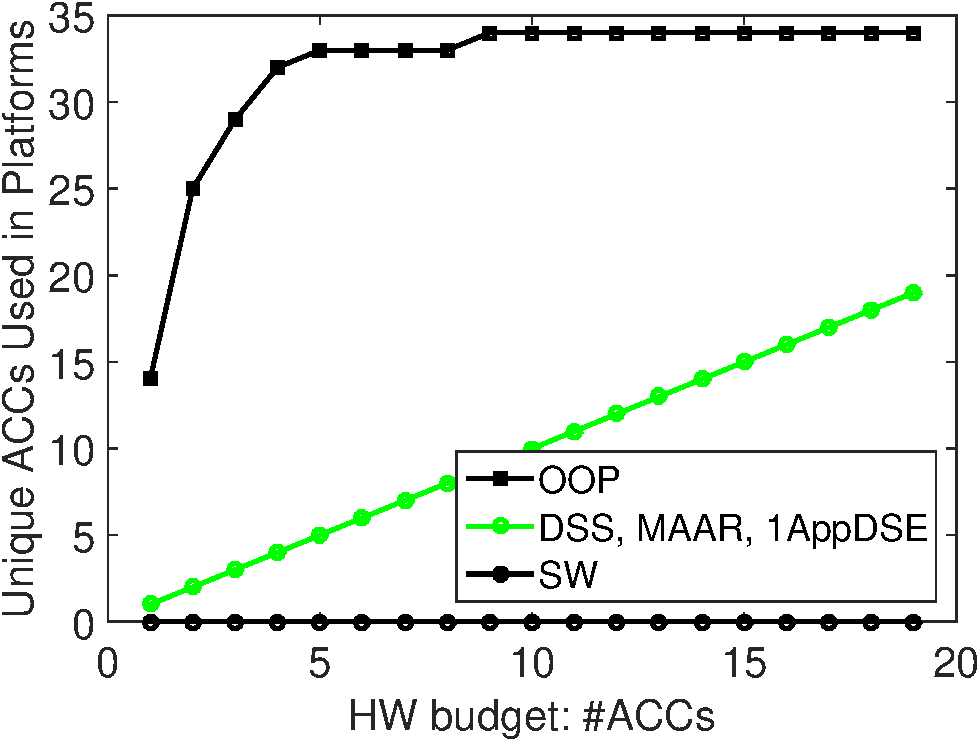
\includegraphics[width=\linewidth]{fig/oopHW.pdf}
	\end{center}
	%\vspace{-8pt}
	\caption{Unique ACCs Used in Platform(s)}
	\label{fig:oopHW}
	%\vspace{-4pt}
\end{wrapfigure}


\figref{fig:oopHW} lists the number of unique ACCs \newtext{ in platform(s) for each DSE}
(SW is empty; DSS, MAAR and 1AppDSE are equal to the budget). OOP has one platform per application, so there are 40 platforms for all applications. Each OPT platform has a number of ACCs equal to the budget, so there are a large number of unique ACCs \newtext{for all OPT platforms}. When each OPT platform has 1 ACC, there are 14 unique ACCs, indicating some reuse. However, if each OPT platform has 2 ACCs, there are 25 unique ACCs (11 more) showing the limits of reuse. This also shows limits of composability of single App DSE. In \figref{fig:alloop}, the MAAR with a 2 ACCs budget allocates \emph{Custom Convlution} and \emph{Canny Edge Detector} kernels, and achieves 67\% the average energy efficiency of OOP, which uses 25 unique ACCs in OOP. This shows a MAAR accelerating a small number of high-computing kernels can achieve good energy efficiency across many applications.

\endgroup

% the order of kernel in OpenVX allocation. CustomConvolution CannyEdgeDetector HarrisCorners OpticalFlowPyramid(LK)  BoxFilter GaussianFilter